%% capitulos/metodologia.tex
%% Capítulo 3 — Metodologia

\chapter{Metodologia}
\label{ch:metodologia}

Este capítulo descreve o protocolo experimental adotado para investigar a
evolução da complexidade estatística dos pesos da camada densa de redes
neurais profundas durante o treinamento. A exposição segue do dado bruto às
medidas: o conjunto de dados (Seção~\ref{sec:dados}), as arquiteturas
(Seção~\ref{sec:arquitetura}) e o protocolo de treinamento
(Seção~\ref{sec:treinamento}); os regimes de treinamento comparados
(Seção~\ref{sec:regimes}); a camada densa como objeto de medida e a
ordem de achatamento dos seus pesos (Seção~\ref{sec:camada-densa}); as
medidas de complexidade (Seção~\ref{sec:medidas}); e o monitoramento durante o
treinamento (Seção~\ref{sec:monitor}).

% ===========================================================================
\section{Conjunto de dados}
\label{sec:dados}

Utiliza-se o MedNIST, conjunto de imagens médicas em escala de cinza,
$64 \times 64$ pixels, distribuídas em seis classes: tomografia abdominal
(\emph{AbdomenCT}), ressonância de mama (\emph{BreastMRI}), tomografia de
tórax (\emph{ChestCT}), radiografia de tórax (\emph{CXR}), radiografia de mão
(\emph{Hand}) e tomografia de crânio (\emph{HeadCT}). Emprega-se a partição
oficial do conjunto em treinamento, validação e teste, com
\num{47164}, \num{5895} e \num{5895} imagens, respectivamente. A semente que
define a partição é fixa em todas as execuções e distinta da semente de
inicialização dos pesos, de modo que todas as execuções compartilham
exatamente os mesmos conjuntos de validação e de teste. O conjunto de teste é
avaliado uma única vez por execução, ao final do treinamento.

% ===========================================================================
\section{Arquiteturas}
\label{sec:arquitetura}

Adota-se a ResNet-18 \cite{he2016} (implementação \texttt{torchvision},
sem pré-treinamento), com a camada totalmente conectada final substituída
para as seis classes do MedNIST. Esta arquitetura totaliza
aproximadamente $11{,}2$ milhões de parâmetros distribuídos em
\textbf{41 tensores com parâmetros aprendíveis}: 20 camadas convolucionais
(\texttt{Conv2d}), 20 camadas de \emph{batch normalization}
(\texttt{BatchNorm2d}) e 1 camada totalmente conectada (\texttt{Linear}),
que é o objeto das medidas deste trabalho
(Figura~\ref{fig:resnet-overview}).

\begin{figure}[H]
  \centering
  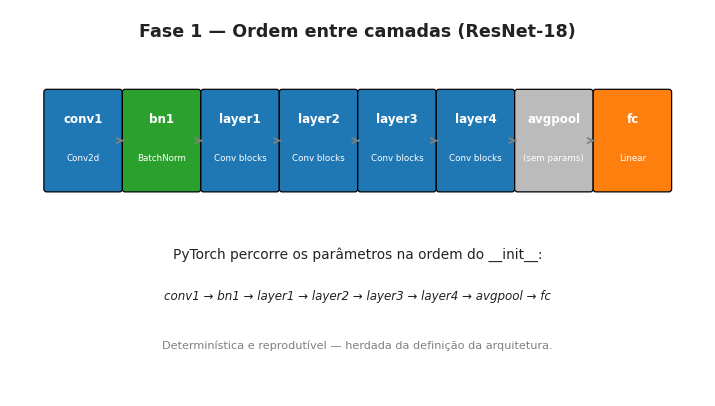
\includegraphics[width=0.95\linewidth]{figures/fig_resnet18_overview.png}
  \caption{Estrutura de nível superior da ResNet-18: oito módulos
  nomeados em sequência. As caixas indicam o tipo de camada
  (azul: Conv2d; verde: BatchNorm2d; cinza: sem parâmetros; laranja: Linear).
  As caixas \texttt{layer1}--\texttt{layer4} são contêineres
  \texttt{Sequential} de blocos residuais.}
  \label{fig:resnet-overview}
\end{figure}

Para descrever o comportamento das medidas em uma segunda arquitetura,
repetem-se as execuções de controle com a DenseNet-121 (implementação
\texttt{torchvision}, sem pré-treinamento), com a camada classificadora
igualmente substituída para seis classes.

% ===========================================================================
\section{Protocolo de treinamento}
\label{sec:treinamento}

O treinamento emprega o otimizador AdamW com taxa de aprendizado $10^{-3}$ e
\emph{weight decay} nulo, entropia cruzada como função objetivo, lotes de 128
imagens e 60 épocas, sem aumento de dados, salvo quando o regime exige outro
número de épocas (Seção~\ref{sec:subamostragem}). O \emph{weight decay} e o
aumento de dados são desligados deliberadamente: ambos são formas de
regularização, e mantê-los atribuiria a diferença entre regimes a mais de uma
causa. Todas as execuções compartilham essa configuração, de modo que cada
regime difere do controle apenas pelo fator manipulado.
Os experimentos foram executados em GPU (\emph{torch} $2{,}4{,}1$ e
\emph{torchvision} $0{,}19{,}1$).

% ===========================================================================
\section{Regimes de treinamento}
\label{sec:regimes}

As trajetórias das medidas são comparadas entre três regimes, todos com a
configuração da Seção~\ref{sec:treinamento}. Em cada regime, a semente que
governa a inicialização dos pesos varia entre as execuções, enquanto a partição
permanece fixa. Validação e teste nunca são alterados: o fator manipulado
incide \emph{apenas} sobre o treino, de modo que a validação mede o efeito
desse fator sobre a generalização.

\subsection{Controle}
\label{sec:controle}

O controle usa o conjunto de treino completo (\num{47164} imagens), com rótulos e
imagens intactos, por 60 épocas, o que corresponde a \num{22140} passos de
otimização (369 lotes por época). Na ResNet-18 há oito execuções de controle;
na DenseNet-121, cinco.

\subsection{Subamostragem do conjunto de treino}
\label{sec:subamostragem}

Treina-se com uma fração $f \in \{\SI{10}{\percent};\ \SI{2}{\percent};\
\SI{1}{\percent}\}$ do conjunto de treino, isto é, \num{4717}, \num{944} e
\num{471} imagens, com cinco sementes por fração. Reduzir o treino diminui
simultaneamente a quantidade de informação e a diversidade dos exemplos, e
torna o sobreajuste mais provável.

A subamostragem traz, porém, uma armadilha que precisa ser controlada.
Experimentos preliminares mostraram que, com poucos passos de otimização, as
estatísticas móveis das camadas de normalização em lote não convergem, e o
modelo colapsa em modo de avaliação --- inclusive sobre o próprio conjunto de
treino. O quadro se parece com sobreajuste catastrófico, mas o mesmo modelo
acerta cerca de \SI{94,5}{\percent} da validação quando a normalização usa as
estatísticas do lote corrente. Mede-se, nesse caso, um artefato de
normalização, e não perda de generalização.

Por isso cada fração é treinada em duas versões. Na versão \emph{curta}, o
número de épocas é o usual para a fração (60 épocas a \SI{10}{\percent} e 200
épocas a \SI{2}{\percent} e \SI{1}{\percent}, ou \num{2220}, \num{1600} e
\num{800} passos). Na versão de \emph{passos igualados}, o número de épocas é
ampliado até que o total de passos iguale o do controle (599, \num{2768} e
\num{5535} épocas, cerca de \num{22140} passos). A comparação entre as duas
versões separa o efeito de ter poucos dados do efeito de ter poucos passos.

\subsection{Ruído nas imagens de treino}
\label{sec:ruido-imagem}

Soma-se às imagens de treino um campo de ruído gerado no domínio da
frequência. Sorteia-se ruído branco gaussiano do tamanho da imagem, aplica-se a
transformada de Fourier bidimensional, multiplica-se o espectro pelo filtro
radial $1/f^{\beta/2}$, com $f$ a frequência espacial, e retorna-se ao domínio
espacial. O espectro de potência resultante é proporcional a $1/f^{\beta}$:
$\beta = 0$ produz ruído \emph{branco}, de potência plana, e $\beta = 1$
produz ruído \emph{rosa}, com mais potência nas baixas frequências. O
componente de frequência nula é zerado, para que o ruído não desloque o brilho
médio da imagem, e o campo é normalizado para desvio-padrão unitário. A imagem
ruidosa é $\mathrm{clip}(x + \sigma z,\ 0,\ 1)$, com $x$ a imagem em $[0, 1]$, $z$
o campo de ruído e $\sigma \in \{0{,}05;\ 0{,}1;\ 0{,}2\}$ a intensidade, na
mesma escala do pixel. O mesmo campo é somado aos três canais, pois o MedNIST é
escala de cinza replicada.

O ruído é \emph{fixo por imagem}: cada imagem de treino recebe sempre o mesmo
campo, em todas as épocas, de modo que a rede pode ajustá-lo. Os rótulos
permanecem intactos. Há cinco sementes por combinação de cor e intensidade,
totalizando 30 execuções.

% ===========================================================================

\section{A camada densa como objeto de medida}
\label{sec:camada-densa}

Seja a camada densa com $M$ entradas $x_1, \dots, x_M$ e $N$ neurônios
$n_1, \dots, n_N$. A matriz de pesos é $W \in \mathbb{R}^{N \times M}$, e
o elemento $w_{ji}$ é o peso do \emph{caminho} $x_i \rightarrow n_j$ ---
convenção que coincide com a forma nativa de \texttt{Linear.weight} no
PyTorch, $[\textrm{out\_features}, \textrm{in\_features}]$.

Como a SampEn$_{1D}$ compara janelas consecutivas, a ordem de achatamento
precisa ser fixada. Duas ordens são naturais. Na ordem \emph{por
neurônio}, percorrem-se todos os pesos que chegam a cada neurônio antes
de passar ao seguinte:

\begin{equation}
    v_{n} = (w_{11}, w_{12}, \dots, w_{1M},\; w_{21}, \dots, w_{2M},\; \dots,\; w_{NM}),
    \label{eq:ordem-neuronio}
\end{equation}

\noindent
o que corresponde ao achatamento nativo, sem transposição. Na ordem
\emph{por entrada}, percorrem-se todos os pesos que partem de cada
entrada:

\begin{equation}
    v_{x} = (w_{11}, w_{21}, \dots, w_{N1},\; w_{12}, \dots, w_{N2},\; \dots),
    \label{eq:ordem-entrada}
\end{equation}

\noindent
equivalente a transpor $W$ antes do achatamento. A
Equação~\ref{eq:ordem-neuronio} mede a regularidade \emph{dentro do campo
receptivo de cada neurônio}; a Equação~\ref{eq:ordem-entrada} mede a
regularidade \emph{da distribuição de uma mesma entrada entre os
neurônios}. Adota-se a primeira como convenção padrão, por corresponder ao
achatamento nativo do PyTorch. O Apêndice~\ref{ap:exemplo-numerico} ilustra as duas ordens
com um exemplo numérico. Para a complexidade LMC a distinção é
irrelevante, pois a medida depende apenas do histograma dos valores e é
invariante a permutações.

O vetor de viés é excluído da análise: o viés é um deslocamento aditivo
do neurônio, não a ligação entre uma entrada e um neurônio, e portanto
não é um caminho no sentido aqui adotado.

Na ResNet-18 aplicada a seis classes, a camada densa (\texttt{fc}) possui
$6 \times 512 = 3.072$ pesos; na DenseNet-121 (\texttt{classifier}),
$6 \times 1.024 = 6.144$. São quantidades que permitem calcular as medidas
sobre a camada inteira, sem subamostragem.

% ===========================================================================
\section{Medidas de complexidade}
\label{sec:medidas}

Sobre a camada densa de cada época são calculadas as medidas descritas a
seguir. Os parâmetros seguem convenções da literatura citada.

\subsection{Complexidade LMC}
\label{sec:medidas-lmc}

A complexidade estatística LMC \cite{lmc1995} é definida como o produto
da entropia de Shannon \cite{shannon1948} pelo desequilíbrio em relação
à distribuição uniforme:
\begin{equation}
  C_{\mathrm{LMC}}(p) \;=\; H(p) \cdot D(p),
\end{equation}
onde, para um histograma normalizado $p$ com $N$ \emph{bins},
\begin{equation}
  H(p) = -\sum_{i=1}^{N} p_i \log_2 p_i, \qquad
  D(p) = \sum_{i=1}^{N} \left(p_i - \tfrac{1}{N}\right)^2.
\end{equation}
Adota-se $N = 100$ \emph{bins}. A entropia é computada em bits ($\log_2$)
e o produto $H \cdot D$ é reportado sem normalização adicional. Como a
medida não é normalizada, sua escala depende de $N$, e nenhuma comparação
entre execuções é legítima sem que o número de intervalos seja idêntico.


\subsection{Entropia amostral SampEn$_{1D}$}
\label{sec:medidas-sampen}

A entropia amostral \cite{richman2000,pincus1991} é definida como
\begin{equation}
  \mathrm{SampEn}(U, m, r) \;=\;
  -\log \frac{A^{m+1}(r)}{B^{m}(r)},
\end{equation}
onde $U$ é o vetor de pesos achatado, $m$ é o comprimento das
sub-sequências comparadas e $r$ é a tolerância de similaridade. As
quantidades $A^{m+1}$ e $B^{m}$ contam pares de sub-sequências cuja
distância de Chebyshev é menor ou igual a $r$. Adotam-se os parâmetros
$m = 2$ e $r = 0{,}2\,\sigma(U)$ \cite{yentes2013}, validados pelo
grupo de pesquisa em estudos prévios.


% ===========================================================================

\section{Monitoramento durante o treinamento}
\label{sec:monitor}

As medidas são calculadas \textbf{a cada época, dentro do laço de
treinamento}, e não sobre \emph{snapshots} analisados posteriormente. A escolha
tem razão prática: nas execuções de passos igualados, com milhares de épocas,
guardar os pesos de cada época seria inviável em disco, e o cálculo dentro do
laço dispensa esse armazenamento.

São calculadas por época a complexidade LMC com $N_{bins} = 100$ e a
SampEn$_{1D}$ com $m = 2$ e $r = 0{,}20\,\sigma$.

O custo do monitoramento é baixo, pois incide apenas sobre a camada densa, e pode
ser desativado por opção de linha de comando.
